Hicimos la elecci�n de direcciones de iluminaci�n con el procedimiento explicado en la parte de desarrollo y obtuvimos la matriz {0,4,10} que tiene el minimo numero de condici�n y la matriz {3,4,8} que tiene el m�ximo numero de condici�n. Luego generamos los campos de las normales y obtuvimos los siguientes resultados:

\begin{center}
   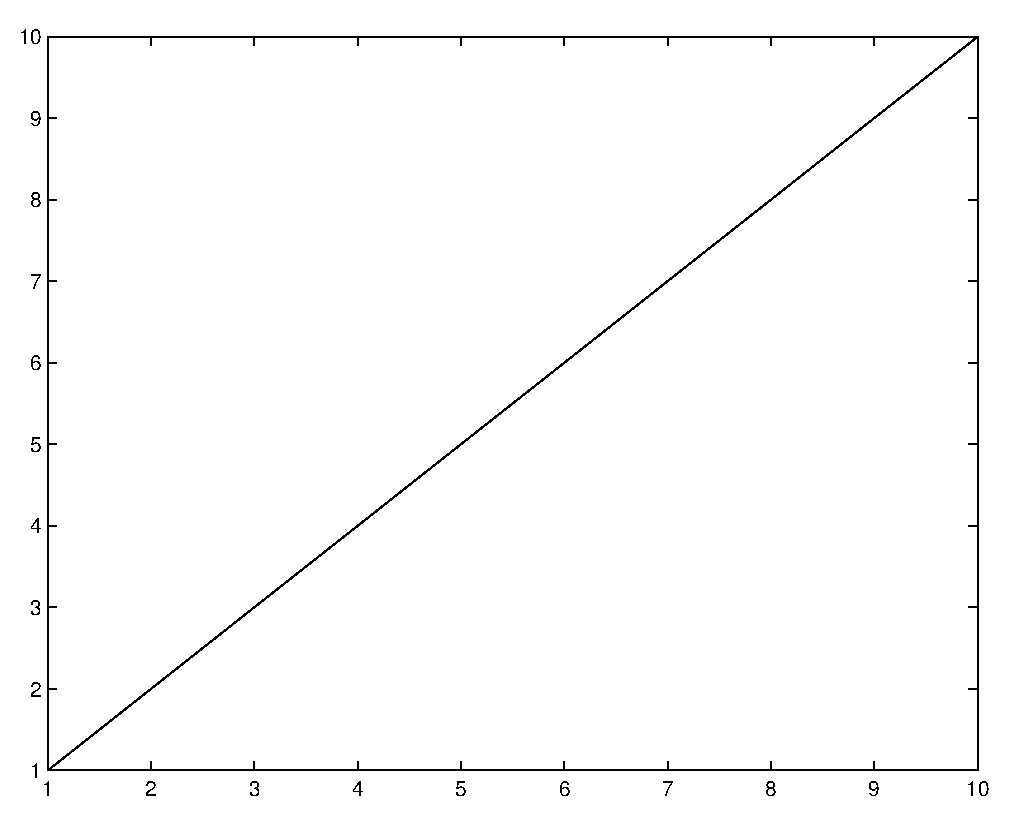
\includegraphics[scale=0.6]{epsFig.eps}
\end{center}